\documentclass[conference]{IEEEtran}
\usepackage{graphicx}
\usepackage{epstopdf}
\usepackage[utf8]{inputenc}
\usepackage{amsmath, amsfonts, amssymb}
\usepackage{float}
\usepackage[portuguese]{babel}
\usepackage {hyperref}
\usepackage{indentfirst}
\usepackage{placeins}
\usepackage[]{algorithm2e}
\usepackage{setspace}
\usepackage{color}
\renewcommand{\rmdefault}{ptm}
\setlength{\parindent}{1cm} 

\newcommand{\Fix}[1]{\textbf{[[}{\color{red} #1}\textbf{]]}}
\newcommand{\Anonim}[2]{#1}
\newcommand{\ie}{i.e.}
\newcommand{\eg}{e.g.}
\newcommand{\cf}{cf.}
\newcommand{\etal}{et al.}

\definecolor{bs}{rgb}{0.59, 0.0, 0.09}

\newcommand{\Davino}[1]{\textbf{[Davino:[}{\color{bs} #1}\textbf{]]}}
\newcommand{\Victor}[1]{\textbf{[Victor:[}{\color{bs} #1}\textbf{]]}}

\newcommand{\cmark}{\ding{51}}%
\newcommand{\xmark}{\ding{55}}%


\begin{document}
\title{Otimização de uma Rede V2V Através de uma Abordagem Multi-Objetiva}

\author{\IEEEauthorblockN{Davino Mauro Tenório da Silva Júnior}
\IEEEauthorblockA{Centro de Informática\\
Universidade Federal de Pernambuco\\
Email: dmtsj@cin.ufpe.br}
\and
\IEEEauthorblockN{Victor Hugo Sabino dos Santos Aráujo}
\IEEEauthorblockA{Centro de Informática\\
Universidade Federal de Pernambuco\\
Email: vhssa@cin.ufpe.br}}

\maketitle

\begin{abstract}

\end{abstract}

\section{Introdução}

Os Sistemas de Transporte Inteligentes (ITS), de acordo com [1], lidam com as questões de tráfego como congestionamento e disseminação de informações, e estão cada vez mais em destaque com o avanço das tecnologias de comunicação sem fio e de automóveis. As Redes \textit{Ad-Hoc} Veiculares (VANETs), que derivam das redes \textit{Ad-Hoc} Móveis (MANETs), permitem que veículos em movimento estejam conectados e se comuniquem sem fio. Esta comunicação pode ser entre dois veículos (V2V) ou entre um veículo e uma infraestrutura (V2I) [2].

Para estabelecer uma comunicação segura e eficiente entre veículos, é necessário que haja uma infraestrutura de comunicação adequada. O padrão IEEE 802.11p apresentado em [3] de Comunicação Dedicada de Curto Alcance (DSRC) foi desenvolvido especificamente para requisitos das VANETs como: auto-organização, configuração automática, topologia dinâmica e alta mobilidade.

Para que a comunicação sem fio opere em tempo real, existem restrições associadas que precisam ser gerenciadas na camada física, como: o tempo de disseminação de dados (\textit{delay}), a perda de pacotes e a taxa de transferência (\textit{throughput}). [4] diz que para garantir um desempenho otimizado em tempo real, é necessário que ambas as restrições sejam atendidas simultaneamente, o que não é trivial devido à limitação de banda e o ambiente veicular altamente dinâmico.

Dentre os vários desafios de VANETs abordados na literatura, [6] destaca o cenário dinâmico e a necessidade de protocolos específicos para redes veiculares que sejam menos afetados pelas frequentes mudanças na rede. [5] aponta o problema de terminal escondido como a principal causa de perda de pacotes em VANETs e propõe uma solução de otimização adaptativa baseada em lógica \textit{Fuzzy} para resolvê-lo. Já [7] faz uma análise do impacto do alcance de trasmissão no desempenho de VANETs em termos de taxa de entrega de pacotes e delay, enquanto [8] relaciona a potência de transmissão de acordo com seu alcance. [5] também destaca a importância de uma janela de contenção dinâmica, que seja otimizada de acordo com o congestionamento no canal. \textbf{[BUSCAR REFERÊNCIA SOBRE A IMPORTÂNCIA DA RELAÇÃO SINAL-RUÍDO MAIS INTERFERÊNCIA]}

As principais contribuições deste artigo são: primeiramente, simular um cenário real de nós em movimento para extrair informações da rede como: \textit{delay}, perda de pacote e \textit{throughput}. Em seguida, definir um espaço amostral de parâmetros de entrada para a simulação, tendo como variáveis a potência de transmissão, o tamanho da janela de contenção ($CW_{min}$ e $CW_{max}$) e a Relação Sinal-Ruído mais Interferência (SINR). Com isso, é possível fazer uma simulação exaustiva com todo o espaço amostral e realizar um estudo comparativo com o resultado obtido através da aplicação de uma técnica de otimização baseada no algoritmo genético multi-objetivo \textit{Fast Non-dominated Sorting Algorithm} (NSGA-II).

O restante do artigo está organizado da seguinte forma: na Seção II, é apresentado o modelo do sistema a ser simulado; na Seção III, é formulado o problema multi-objetivo e apresentado o algoritmo NSGA-II; na Seção IV, é construído o modelo de simulação e a avaliação de seu desempenho; a seção V conclui o trabalho e são discutidos possíveis trabalhos futuros.

\section{Modelo do Sistema}

Neste estudo, é considerado um ambiente urbano comumente encontrado em regiões metropolitanas. A Figura 1 representa o cenário utilizado para a simulação, retirado do \textit{OpenStreetMaps}, o ambiente é localizado no centro da cidade do Recife, nas mediações da Av. Agamenom Magalhães. O número de veículos dentro da rede aumenta conforme o tempo de simulação, e são aleatoriamente colocados no mapa e com velocidade variando de acordo com o tráfego do local, tornando o modelo mais realista. \textbf{[VERIFICAR COMO FOI FEITA A SIMULAÇÃO DO SUMO]}


%%\begin{figure}[h]
 %% \centering
  %%\includegraphics[scale=0.25]{nome_da_imagem.jpg}
  %%\caption{Fragmento da cidade do Recife utilizado no cenário}
  %%\label{fig:how_pop3_works}
%%\end{figure}

Assume-se que todos os veículos estão equipados com uma Unidade de Controle de Bordo (OBU), que dá suporte a comunicações V2I e V2V. Adicionalmente, os veículos são capazes de transmitir e receber informações atualizadas enquanto trafegam sobre o tráfego, acidentes, e informações baseadas em localização.

\section{Formulação do Problema}
\label{sec:form-problema}

Baseado nas informações anteriores, o objetivo deste estudo é minimizar a perda de pacotes e o \textit{delay} de disseminação, e aumentar o \textit{throughput} de dados de uma rede VANET considerando apenas a comunicação entre veículos (V2V). Portanto, pode-se propor uma técnica de Otimização Multi-Objetiva (MOO) para resolver este problema. A MOO é um campo que diz respeito a otimização de duas ou mais funções objetivas [9]. A solução deste problema envolve a localização de um conjunto de soluções candidatas chamadas de não dominadas. O conjunto de soluções não dominadas ótimas é chamado de pareto ótimo. Todas as soluções que estão no pareto ótimo pertencem ao conjunto de paretos, e os pontos representados em relação a cada objetivo no espaço são chamados de pareto \textit{front}. A complexidade dos problemas MOO são diretamente ligadas as dependências entre as variáveis de decisão em relação a seus objetivos, no caso em que existem conflitos entre estas variáveis, é necessário um \textit{trade-off} para analisar qual objetivo deve ser priorizado.

O presente trabalho adotou o algoritmo genético multiobjetivo denominado \textit{Fast Non-dominated Sorting Genetic Altorithm} (NSGA-II) proposto por [11]. Este algoritmo aplica o conceito de dominância ao classificar elementos da população de maneira elitista em fronteiras (\textit{fronts}), de acordo com o grau de dominância. A cada geração, os indivíduos classificados no primeiro \textit{front} são considerados melhores, ou, dominantes. Após a classificação em \textit{fronts}, os indivíduos também são ordenados através de um operador de diversidade baseado num indicador de densidade (\textit{crowding distance}), que relaciona a distância de cada indivíduo para seus vizinhos imediatos com a distância entre as soluções extremas do mesmo \textit{front}. O pseudocódigo para o NSGA-II é apresentado no Algoritmo 1 a seguir.

\section{Avaliação do desempenho}
\label{sec:avaliacao-desemp}

Neste trabalho, os cenários descritos na seção ~\ref{sec:form-problema} foram simulados utilizando a ferramenta Veins \Davino{ Descrever o veins?} de forma exaustiva, tendo como resultado um arquivo de resultados. Para avaliação do algoritmo multi-objetivo em busca da melhor configuração de parâmetros a serem utilizados no simulador, foi utilizada uma implementação em Ruby do algoritmo NSGA-II com funções objetivo adaptadas para o problema proposto. As funções foram baseadas no problema multi-objetivo introduzido por Schaffer e apresentado em [11], e visam maximizar o \textit{throughput} e minimizar a perda de pacotes e \textit{delay}.

Foi utilizada uma implementação do algoritmo NSGA-II na linguagem de programação Ruby [9], adaptando a mesma para o problema e proposito deste trabalho.

\subsection{Parâmetros de Configuração}
\label{subsec:param-config}

\Davino{Victor, por favor descreve de forma breve os parâmetros utilizados (cwmin, cwmax, slotlength, txpower)}

\paragraph{Simulação}

A representação do indivíduo no algoritmo NSGA-II se dá por um mapa de
16 bits.  Cada indivíduo é dividido de forma a representar os quatro
parâmetros de configuração utilizados no simulador e descritos na
seção ~\ref{subsec:param-config}, a saber (1) $CW_{min}$, (2)
$CW_{max}$, (3) slot length, e (4) txPower, como mostra a figura
~\ref{fig:bits-config}.  A simulação consiste em efetuar o
\textit{parse} desse indivíduo para uma dada configuracão, isto é, um
valor para cada parãmetro, e buscar essa configuração no arquivo
resultante da busca exaustiva. Uma vez encontrados os resultados da
simulação realizada com os parâmetros de configuração do indivíduo,
isto é, \textit{throughput}, perda de pacotes e \textit{delay}, são calculadas as respectivas funções objetivo buscando determinar se o indivíduo é ótimo, isto é, se condizem com os objetivos propostos na
seção ~\ref{sec:avaliacao-desemp}.
O algoritmo NSGA-II busca então pelo pareto \textit{front} com os melhores resultados de simulação para um dado indivíduo (configuração), executando o rankeamento dos paretos não dominados, e os passos de reprodução e \textit{crossover}.

\begin{figure}[h]
  \centering
  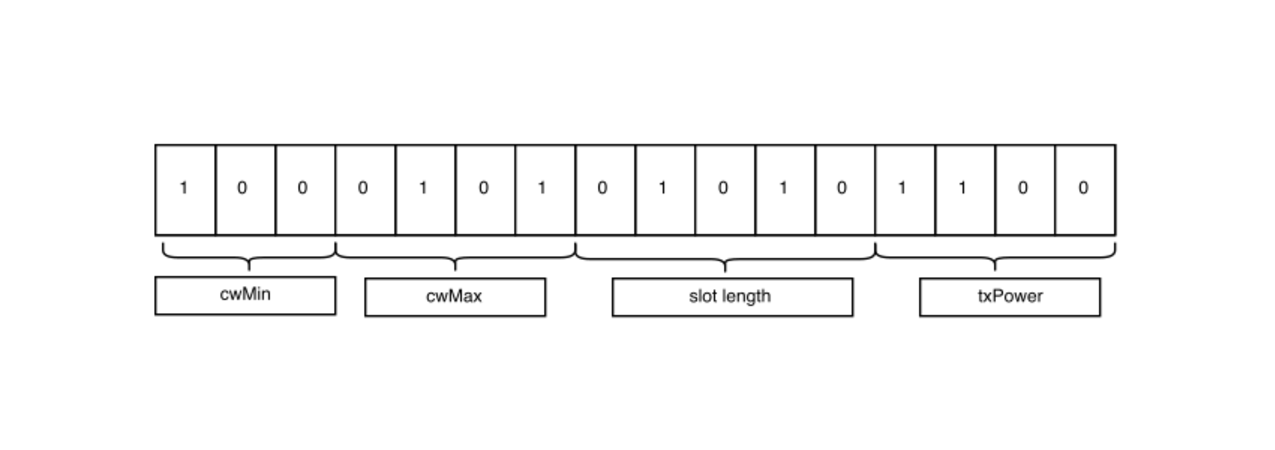
\includegraphics[scale=0.25]{figures/bits-config.pdf}
  \caption{Indivíduo utilizado no algoritmo representando uma dada configuração para simulação.}
  \label{fig:bits-config}
\end{figure}


\paragraph{Resultados}

Para execução do algoritmo NSGA-II, foi utilizada uma taxa de \textit{crossover} de 0.98\%, como consta em [9], bem como 50 gerações.
Foi utilizada uma população de 5 a 50 indivíduos...


\section{Conclusão}

\nocite{*} % Include everything in the .bib file.

%\bibliographystyle{IEEEtran}
%\bibliography{paper}

% that's all, folks
\end{document}
